%%%%%%%%%%%%%%%%%%%%%%%%%%%%%%%%%%%%%%%%%
% Journal Article
% LaTeX Template
% Version 1.0 (25/8/12)
%
% This template has been downloaded from:
% http://www.LaTeXTemplates.com
%
% Original author:
% Frits Wenneker (http://www.howtotex.com)
%
% License:
% CC BY-NC-SA 3.0 (http://creativecommons.org/licenses/by-nc-sa/3.0/)
%
%%%%%%%%%%%%%%%%%%%%%%%%%%%%%%%%%%%%%%%%%

%----------------------------------------------------------------------------------------
%	PACKAGES AND OTHER DOCUMENT CONFIGURATIONS
%----------------------------------------------------------------------------------------

\documentclass[twoside]{article}
\usepackage{etex}
\usepackage{pgfplots}
\usepackage{cite} % Better citations
\usepackage{setspace}
\usepackage{mathtools}
\usepackage[sc]{mathpazo} % Use the Palatino font
\usepackage[T1]{fontenc} % Use 8-bit encoding that has 256 glyphs
\linespread{1.00} % Line spacing - Palatino needs more space between lines
\usepackage{microtype} % Slightly tweak font spacing for aesthetics
\usepackage{graphicx}
%\usepackage[hmarginratio=1:1,top=16mm,columnsep=20pt]{geometry} % Document margins
\newcommand{\bigO}{\ensuremath{\mathcal{O}}}
\usepackage[headsep=0.05in,scale=1.0,margin={0.5in,0.5in},columnsep=20pt]{geometry}
%\oddsidemargin 0.0in %%this makes the odd side margin go to the default of 1inch
%\evensidemargin 0.0in
%\headheight 0.5in
%\topmargin 0.5in
%\textheight 9.0in
%\textwidth 6.5in %%sets the textwidth to 6.5, which leaves 1 for the remaining right margin with 8 1/2X11inch paper 

\usepackage{multicol} % Used for the two-column layout of the document
%\usepackage{hyperref} % For hyperlinks in the PDF

\usepackage[hang, small,labelfont=bf,up,textfont=it,up]{caption} % Custom captions under/above floats in tables or figures
\usepackage{booktabs} % Horizontal rules in tables
\usepackage{float} % Required for tables and figures in the multi-column environment - they need to be placed in specific locations with the [H] (e.g. \begin{table}[H])
\usepackage{lettrine} % The lettrine is the first enlarged letter at the beginning of the text
\renewcommand{\LettrineTextFont}{\rmfamily}
\usepackage{paralist} % Used for the compactitem environment which makes bullet points with less space between them

\usepackage{abstract} % Allows abstract customization
\renewcommand{\abstractnamefont}{\normalfont\bfseries} % Set the "Abstract" text to bold
\renewcommand{\abstracttextfont}{\normalfont\small\itshape} % Set the abstract itself to small italic text

\pagestyle{plain} % no page numbers in footer
\usepackage{scalefnt} %scale font for title
\usepackage{titlesec} % Allows customization of titles
\usepackage{comment}	%Allows addition of comments
%\usepackage[small,compact]{titlesec}
\titleformat{\section}[block]{\large\scshape\centering{\Roman{section}.}}{}{1em}{} % Change the look of the section titles 

%----------------------------------------------------------------------------------------
%	TITLE SECTION
%----------------------------------------------------------------------------------------

%\title{\vspace{-15mm}\fontsize{20pt}{5pt}\selectfont\textbf{Experienced Search}} % Article title

%----------------------------------------------------------------------------------------

\begin{document}
%\title{\vspace{-20mm}{On-Line Recognition of Continuous Mouse Gesture Sequences}}
%\date{}
%\maketitle % Insert title
\scalefont{2}
\centerline{Recognition of Unistroke Gesture Sequences}
\normalsize

%----------------------------------------------------------------------------------------
%	ARTICLE CONTENTS
%----------------------------------------------------------------------------------------

\begin{multicols}{2} % Two-column layout throughout the main article text

\section{Problem Statement}
\lettrine[nindent=0em,lines=2]{G}estures are a popular and growing form of input in human-centric user
interfaces, primarily due to their natural use in everyday communication \cite{mitra_gesture_2007}.
One important domain where gestures are frequently seen is law enforcement.
Of particular concern to law enforcement
agencies is recognition of gang symbols in grafitti and other forms of
hand-written communication. The United States Federal Bureau of Investigation's
Safe Streets and Gang Unit commonly encounters handwritten communication
using custom gestures\cite{lyddane_donald_united_2006}. In this scenario,
gesture recognition is difficult due primarily to 1) the relatively small number
of identified samples (i.e., lack of training data) and 2) the nature of the
communication, which is often an unbroken string of symbols and characters
(i.e., a continuous gesture sequence), 3) the separation of
knowledge among law enforcement divisions, which necessitates a recognition approach comparing communication against a database of identified symbols
associated with gang activity, and 4) the creation and use of custom gestures.

Recognizing a sequence of gang symbols is primarily difficult due to the
segmentation problem: identifying where one symbol ends and another begins in
order to match each unknown symbol against a database.
Note that unlike a written language, the sequence of symbols/gestures doesn't
follow a well-defined grammar. Moreover, the sequence typically has no obvious
separation of symbols, similar in nature to cursive handwriting. In the next section,
we review work related to this problem. 
%To our knowledge, this problem has not been addressed in the literature.

%Problem addressed and its importance
%    ⁃    poor: does not mention problem or does not say why it is important
%    ⁃    acceptable: problem is tied to societal needs and backed up with reasons
%    ⁃    exceptional: succeeds in really convincing the reader (way beyond lip service)

%------------------------------------------------
\section{Related Work}

Much of the related work focuses on recognition using a ``gesture grammar" (e.g., language grammar).
Yang et al \cite{yang_gesture_1994} present work on recognition of individual
gestures in continuous gesture sequences, with the notable difference between
their work and ours being that they train on gesture sequences defined \textit{a
priori}, as well as an extensive training period, both of which we see
as deficiencies.

Hong et al, in their paper on Chinese character recognition 
\cite{hong1998segmentation}, use a two-level iterative segmentation technique that uses
whitespace separation to split character sequences into individual characters.
Their approach does not work for our problem, where gestures are drawn in one continuous motion,
uninterrupted by white space.

The \$1 recognizer \cite{wobbrock2007gestures} is a single gesture
recognition system which works even without any training by the user (the system has a built-in gesture set which can be extended for personalized recognition). The primary
deficiency of this system is its inability to recognize sequences of gestures.

%------------------------------------------------
\section{Approach}

In order to study the problem of segmentation of a gesture sequence,
we created a web-based prototype of a gesture recognition environment using mouse-based input, inspired by (and derived from) the \$1 recognizer web-based application\cite{wobbrock2007gestures}. 
The user chooses from a list of custom gestures, trains the system by drawing the individual gestures,
and then draws 1, 2, or 3 arbitrary gestures comprising a single unistroke. During recognition,
the system attempts to segment the unistroke into the correct gestures, as shown in the following figure.

\begin{figure}[H]
	\centering
	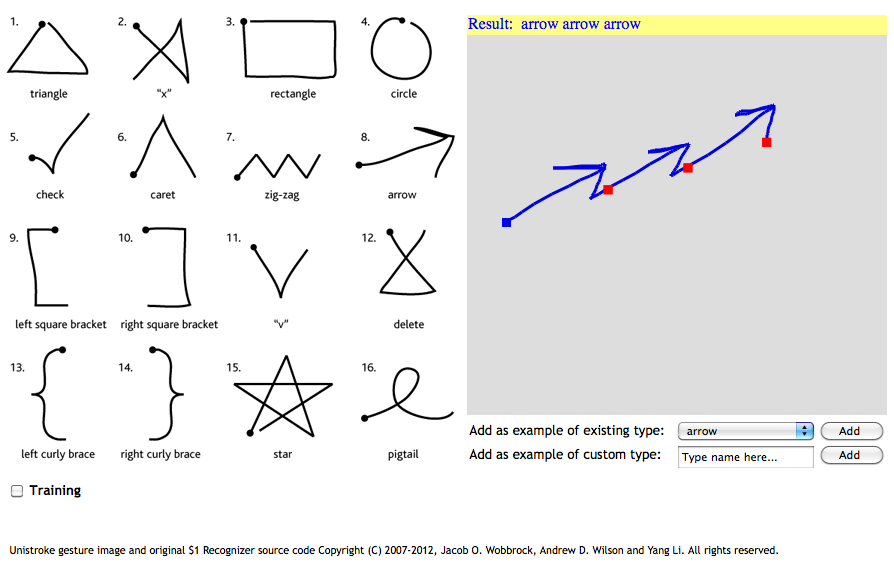
\includegraphics[height=6cm, width=9cm]{Images/GUI.png}
	\label{fig1}
	\caption{Recognition GUI}
\end{figure}
  
%We are focused on creating a quick and flexible prototyping environment, in which the user
%trains the system on individual mouse gestures. However the user can then create custom unistroke
%gesture sequences, which will be segmented into individual gestures and identified. The main goal
%of this project is to get an efficient recognition system up-and-running in the 
%shortest possible time without the need to excessively train it. 

Our approach, at a high level, is very straightforward, and divided into two
main steps. The first step is to match each individual gesture against a portion
of the input data. The second step is to remove the first gesture from the input
sequence and iterate, searching for additional gestures.
The difficult part is accurately recognizing which of the individual gestures
appears first in the unistroke sequence.

In our approach, we categorize the gesture sequence given as input by the user
as a set of candidate points, which need to be matched against one or more sets
of template points, in order to spot a gesture. The main challenge in our
approach was to come up with a technique which was neither too strict (as users
generally cannot repeat the exact same pattern again and again) nor too lenient
(we do not want to recognize some random squiggle as any particular gesture).
There are two stages in the recognizer, (a) A brief training stage where the
user draws a particular gesture and adds its model to the list of
``recognizable'' gestures (b) A recognition phase where the user can draw any
sequence of gestures, from which those that have a corresponding model in the
system will be recognized.

\subsection*{Training Phase}

Depending on the speed at which a gesture is drawn, there can be a lot of
variance in the number of input points to be considered as part of the template.
For this reason, irrespective of the number of raw pixels drawn by the user, we
quantize it into N equidistant points, where N=64 proved to give adequately
accurate as well as computationally inexpensive results. The user is required to
give a name for this gesture. For each of the labeled gesture, we find its
\textit{indicative angle} \cite{wobbrock2007gestures}, which is the angle
subtended between the first point and the centroid of the gesture. We define the
centroid of a gesture to be the point which has the maximum density of
neighboring pixels. If the user draws more instances of the same gesture, the
centroid will be computed as an average over all the instances. However, we have
found that even with very few instances of each gesture (sometimes even just 1),
we get a high accuracy rate for recognizing one or more individual gestures.

\subsection*{Recognition Phase}
As stated previously, the foremost challenge in our project was that of
segmenting the input sequence in order to obtain the correct number of gestures
drawn by the user. In addition, since users are not constrained at the time of
defining new gestures, ambiguity can exist based on where a gesture sequence is
segmented. Figure 1 depicts this problem of ambiguity. However in our approach
we concern ourself only with the first problem; we consider either one of these
two possibilities to be correct.

\begin{figure}[H]
	\centering
	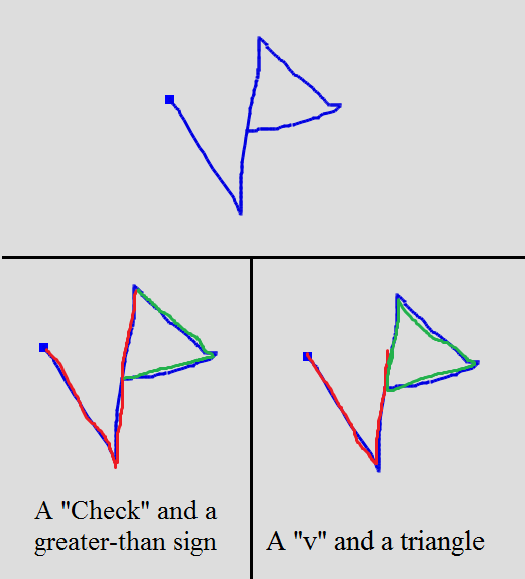
\includegraphics[height=5cm, width=5.5cm]{Images/Ambiguity1.png}
	\label{fig1}
	\caption{Ambiguity in gesture recognition after}
\end{figure}

We obtain the raw pixels which are part of the gesture sequence drawn by the
user. We pick out the first 64 equidistant points (the candidate points) in the
input sequence and find its centroid and the \textit{indicative angle}. This
subset of points is rotated by the \textit{indicative angle} and is scaled to
fit into a square of fixed dimensions. This step is then repeated for all the
gesture models recorded into the system by the user. It is necessary to fit both
the template points as well as the candidate points into a fixed square in order
to make the recognizer invariant to scale. For each predefined gesture, we
calculate the euclidean distance between each template point T[k] and the
candidate point C[k] and average it over the 64 points. Equation 1 computes this
distance:

\[
 d_k = \frac{\displaystyle\sum\limits_{k=1}^N \sqrt{(C[k]_x-T[k]_x)^2 + (C[k]_y-T[k]_y)^2}}{N}
\]

This way we have obtained a ``distance'' measure for the input points with
respect to each of the predefined gestures. However, it would be incorrect to
simply pick the gesture which gives the lowest distance, as this might give a
drastically incorrect result. So we keep reading pixels from the raw input, in
groups of 32, and add it to the candidate points. We re-evaluate this distance
measure for the new set of points. We keep performing this process of ``window
sliding'' until there is a value of $d_k$ which falls below an empirically
determined threshold value. The system then adds the gesture corresponding to
this value of $d_k$ to the list of gestures present in the gesture sequence.
This gesture is then ``spliced'' off from the user input and the above process
is repeated until there are no more points left in the input. The list of
gestures thus obtained corresponds to the individual gestures present in the
gesture sequence. %Figure 2 depicts this algorithm traced out for a sample input
gesture sequence.
%Should there be a diagram here?

Obviously due to the number of computations involved at every iteration of the
window sliding process, its necessary to have a limit on the number of input
gestures. We have performed our evaluations by defining 16 gestures, but we
believe that this can go upto 50 and the recognizer will still give a reasonable
performance. %Justification?

%------------------------------------------------
\section{Evaluation}

We have evaluated the system on three parameters:
\begin{enumerate}
	\item Accuracy of the recognition system: This is an all-or-nothing measure. For input sequence of lengths 1, 2 or 3, we measured the number of times our system got all the gestures in the input correctly.
	\item Segmentation efficiency: We have tried to quantify the efficiency of our segmentation routine by finding out the number of instances in which the system has segmented the gesture sequence into the correct \emph{number} of gestures. Even if the system recognizes one or more of the gestures wrongly, if it manages to report the correct number of individual gestures, we consider that to be a positive result for this metric.
	\item Relaxed gesture recognition accuracy: This is a relaxed version of the first metric. This parameter will not take into consideration the ordering of the gestures in the input sequence and will also consider partially recognized sequences as favorable. For instance, if the user has drawn a "check" followed by a "star" and the program reports it as a "star" and "arrow", this metric will give it a score of 1/2. That is, the score assigned to a particular solution provided by the system is:
	\[
		Relaxed Accuracy = \frac{\text{Reported gestures in the input}}{\text{Total gestures in the input sequence}}
	\]
Obviously this measure will be different only for input sequences of length greater than 1.
\end{enumerate}
The results of these three metrics were obtained from a micro-study involving a single third-party user and are represented as a percentage in Tables 1,2 and 3 respectively. 20 trials were performed each for input of lengths 1,2 and 3.

\begin{table}[H]
  \centering
  \caption{Accuracy rate of the system for a given input length}
    \begin{tabular}{rr}
    \toprule
    Sequence Length & Accuracy Rate \\
    \midrule
    1     & 90\% \\
    2     & 50\% \\
    3     & 20\% \\
    \bottomrule
    \end{tabular}%
  \label{tab:addlabel}%
\end{table}%

\begin{table}[H]
  \centering
  \caption{Segmentation accuracy of the system for a given input length}
    \begin{tabular}{rr}
    \toprule
	Sequence Length & Segmentation Accuracy \\
    \midrule
    1     & 100\% \\
    2     & 80\% \\
    3     & 60\% \\
    \bottomrule
    \end{tabular}%
  \label{tab:addlabel}%
\end{table}%

\begin{table}[H]
  \centering
  \caption{Relaxed Accuracy rate of the system for a given input length}
    \begin{tabular}{rr}
    \toprule
    Sequence Length & Accuracy Rate \\
    \midrule
    2     & 50\% \\
    3     & 50\% \\
    \bottomrule
    \end{tabular}%
  \label{tab:addlabel}%
\end{table}%

\begin{figure}[H]
	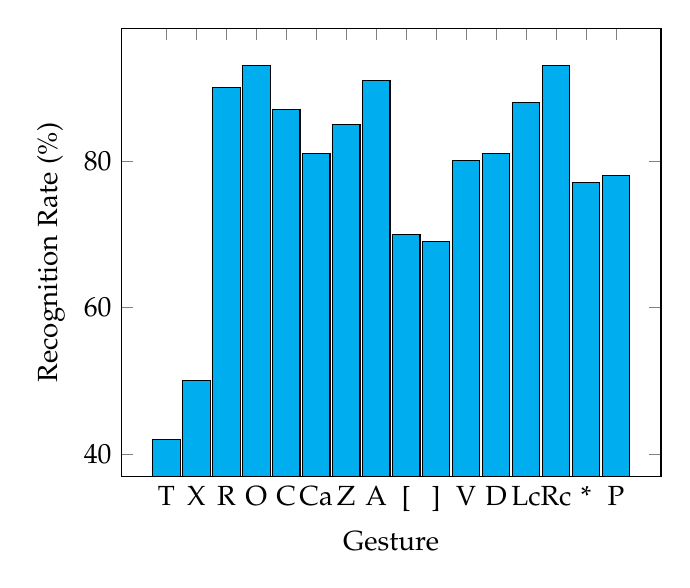
\begin{tikzpicture}
        \begin{axis}[
            symbolic x coords={T, X, R, O, C, Ca, Z, A, [, ], V, D, Lc, Rc, *, P},
            xtick=data, ylabel=Recognition Rate (\%), xlabel=Gesture
          ]
            \addplot[ybar,fill=cyan] coordinates {
                (T,   42)
                (X,  50)
                (R,   90)
                (O,   93)
                (C,   87)                
                (Ca,   81)
                (Z,   85)
                (A,   91)
                ([,   70)
                (],   69)
                (V,   80)
                (D,   81)
                (Lc,   88)
                (Rc,   93)
                (*,   77)
                (P,   78)
            };
        \end{axis}
    \end{tikzpicture}
	\caption{Recognition rates for individual gestures}
	\label{fig2}
\end{figure}	

Also we were interested to find out the recognition rate for each of the predefined gestures individually. This is represented in Figure 2. 

In Figure 3, the time taken for segmenting and recognizing gestures is plotted for different number of predefined gestures (``Gesture Library'').

\begin{figure}[H]
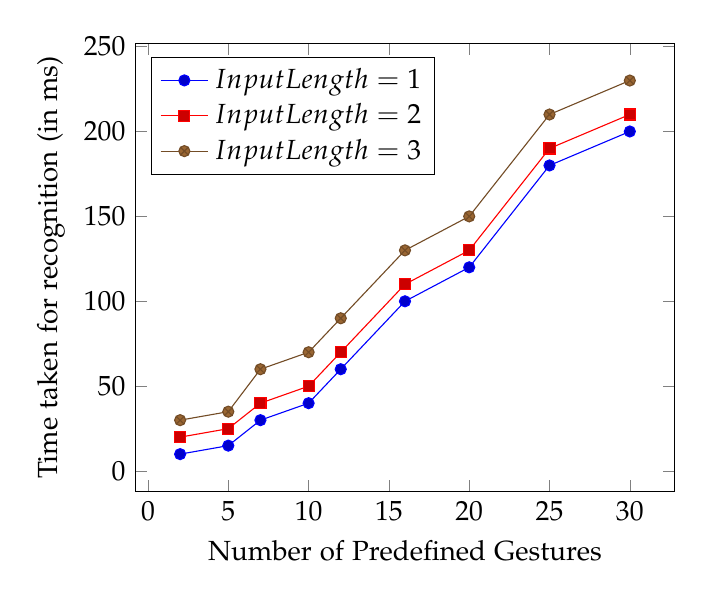
\begin{tikzpicture}
    \begin{axis}[
	    legend pos=north west,
        xlabel=Number of Predefined Gestures,
        ylabel=Time taken for recognition (in ms)
    ]
      \addplot plot coordinates {
        (2,     10)
        (5,    15)
        (7,    30)
        (10,   40)
        (12,   60)
        (16,   100)
        (20,  120)
        (25,  180)
        (30,  200)
    };

      \addplot plot coordinates {
        (2,     20)
        (5,    25)
        (7,    40)
        (10,   50)
        (12,   70)
        (16,   110)
        (20,  130)
        (25,  190)
        (30,  210)
    };
    
      \addplot plot coordinates {
        (2,     30)
        (5,    35)
        (7,    60)
        (10,   70)
        (12,   90)
        (16,   130)
        (20,  150)
        (25,  210)
        (30,  230)
    };
    \legend{$Input Length=1$\\$Input Length=2$\\$Input Length=3$\\}
    \end{axis}
\end{tikzpicture}	
	\caption{Time taken for segmenting and recognizing gesture sequences}
	\label{fig3}
\end{figure}

Figure 4 is a plot of the variation of the recognition rate with respect to the number of times each predefined gesture was drawn during the training phase. Each of the gesture in the ``Gesture Library'' were trained equally, and this is represented by the x-axis of the plot.

\begin{figure}[H]
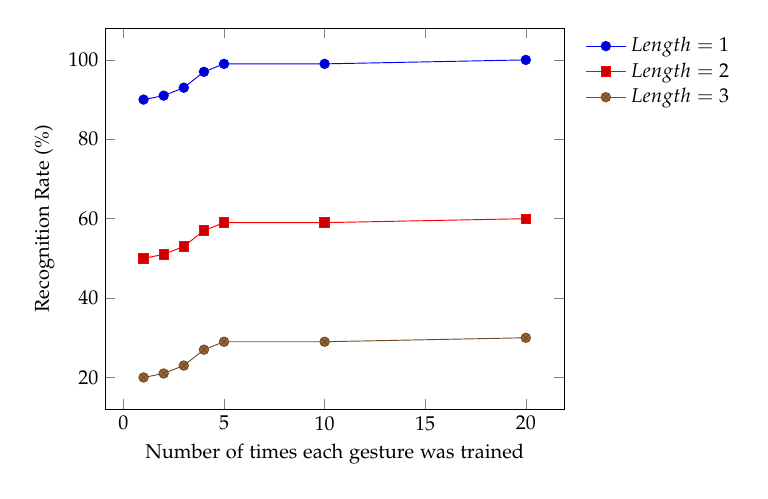
\begin{tikzpicture}[thick,scale=0.85, every node/.style={scale=0.85}]
    \begin{axis}[
	    legend pos= outer north east,
	    legend style={draw=none},
        xlabel=Number of times each gesture was trained,
        ylabel=Recognition Rate (\%)
    ]
      \addplot plot coordinates {
        (1,     90)
        (2,    91)
        (3,    93)
        (4,   97)
        (5,   99)
        (10,   99)
        (20,  100)
    };

      \addplot plot coordinates {
        (1,     50)
        (2,    51)
        (3,    53)
        (4,   57)
        (5,   59)
        (10,   59)
        (20,  60)
    };

      \addplot plot coordinates {
        (1,     20)
        (2,    21)
        (3,    23)
        (4,   27)
        (5,   29)
        (10,   29)
        (20,  30)
    };
    
    \legend{$Length=1$\\$Length=2$\\$Length=3$\\}
    \end{axis}
\end{tikzpicture}	
	\caption{Recognition Rate Vs. Size of Training Data}
	\label{fig4}
\end{figure}

%------------------------------------------------
\section{Discussion}

From Tables 1, 2 and 3 it is apparent that the method of progressively applying
dynamic time warping over the input sequence of points gives fairly average
results. It is clear that the process of geometric matching works much better
for recognizing individual gestures than for gesture sequences. However, it is
noteworthy to observe that our algorithm was able to segment the input sequence
correctly, on an average, about 80\% of the time. There was no case where the
user drew just one gesture and our system reported it to be more than one. This
complete absence of a ``false positive'' is an encouraging sign, which leads us
to believe that our segmentation routine is robust. Although the trials were
conducted by only one person, we discovered that our system was fairly invariant
to spatio-temporal factors. In such problems, author bias tends to play a big
role, and hence we would have got a more complete picture had we been able to
test it with multiple users. The results from Table 3 indicate that 75\% of the
time the system is able to correctly recognize atleast one gesture in sequences
of length greater than 1. This is a significant achievement considering how
little training is required to get the system up-and-running.

From Figure 2 it is possible to obtain gestures which are ``easily
recognizable'' or in other words ``easily distinguishable'' from one another (by
simply picking out the gestures with the highest recognition rates).
%Confusion matrix
The purpose of this exercise was to find out a set of gestures which are very
different from one another. If the input were restricted to sequences composed
of only these allowable gestures, we posit that we can obtain a much higher
recognition accuracy by using the same algorithm.

The need to have a restricted set of gestures as part of the input is also
justified by the results compiled in Figure 3. It shows that there is almost a
linear relationship between the number of predefined gestures and the time taken
to segment and recognize individual gestures in an input sequence. This is
understandable since every iteration of the segmentation routine compares the
candidate points with all template models available to the system. Therefore by
fixing the number of possible gestures, we can obtain a fairly good (and
constant) estimate for an upper limit on the time complexity for the recognition
process, for a input sequence of a given length.

Figure 4 shows that we do not require a lot of training data to get a good
recognition rate. Even if each gesture has just one template instance during the
training phase, we were able to achieve 90\%, 50\% and 20\% recognition accuracy
for 1-gesture, 2-gesture and 3-gesture input sequences. Also we observe that by
increasing the number of training samples, we were able to improve on the
accuracy, but this improvement was incremental most of the time. It goes to show
that the role of the training phase in our approach is minimal.

We considered using the HMM approach for solving our problem. In order to
recognize gesture sequences, we would have had to construct HMMs for each of the
individual gestures. Then we can build (not by training, but programatically)
models of all possible 2-gesture sequences from our ``Gesture Library'' by
simply chaining the various permutations of the available gestures. %Needs more clarity here.
For instance, if the number of predefined gestures is 4, and the input sequence
is of length 2, then we would have 4 HMMs for the individual gestures and $4^2$
HMMs for all possible 2-gesture sequences. We could then simply run the features
extracted from the candidate points through each of these HMMs and get the
result in a similar manner as Yang et al. However, this solution suffers from
combinatorial explosion and will not scale well to handle longer input
sequences. For instance, consider the system to have $M$ predefined gestures and
an input sequence which is $N$ gestures long. Then the number of HMMs which need
to be constructed in this case, which will give a good approximation of the time
complexity of this approach, is
\[
	M + M^2 + M^3 + ... + M^N = \bigO{(M^N)}
\]

However our approach, as proven by the results of Figure 3, has a time
complexity = \bigO{(M*N)}, which is far less computationally demanding.
Nonetheless, we have compared our results with some approaches which have used
HMMs in attempting to solve problems similar to ours.

%Comparison with HMM approaches

Tanguay \cite{tanguay_jr_hidden_1995} in his thesis, has performed
identification of lower-case English alphabets and has reported an accuracy of
60-70\% on individual characters after extensive training by extracting 5
features and throwing it at an HMM. In our approach, after adding just one
training sample for each of the lower-case alphabets, individual gesture
recognition was close to 85\%. Again this comparison may not be complete due to
user bias, but it indicates that dynamic time warping is also a feasible
approach in gesture recognition.

Since Tanguay does not recognize multiple gestures in a gesture sequence, we
compare our results with that of Yang et al \cite{yang_gesture_1994}. Although
they do not mention results for gesture sequences of length 3, they report a
really high accuracy rate of upto 99.78\%. Our results from Table 1 are much
less impressive, as we were only able to get 50\% accuracy. However there are
certain key differences in both the approaches. Yang et al train Hidden Markov
models for both individual gestures as well as for all possible 2-gesture
combinations. Moreover, their gesture set is restricted to the numerals 0-9.
Hence in the recognition phase of their approach, they simply pass the raw input
to each of the available HMMs and the gesture(s) corresponding to the model that
gives the highest probability is selected.

From our work we have learnt that the dynamic time warping approach is a good
alternative to HMMs in problems of gesture recognition; more so if computational
power is a constraint. However there is potential for further research and work
to be done in this field. An immediate work for the future is to be able to
carry forward our assumption about a restricted set of input gestures and
implement it. It would be worthwhile in investigating the performance measure of
the system when the possible input sequence is made up of a finite ``alphabet''.
Also, given sufficient computational horsepower, it would be interesting to
construct HMMs for gesture sequences of varying lengths, say upto 5, using the
chaining approach and compare the results with those that we have obtained. A
fundamental constraint of our implementation is that the input needs to be
constructed in one stroke, which does not give much leeway to the user
constructing the gesture sequence. Another potential problem for the future is
to extend this system, allowing the user to input gesture sequences in a more
free-form manner using multiple strokes.

%----------------------------------------------------------------------------------------
\section{References}

\begin{spacing}{0.9}
%\scalefont{0.9}
\bibliographystyle{unsrt}	
%\bibliography{myrefs}
\begingroup
\renewcommand{\section}[2]{}%
\bibliography{myrefs}
\endgroup
\end{spacing}
%\normalsize

\end{multicols}
\end{document}

%	Member #1: Justin Permar - GT ID:902931271
%	Member #2: Arvind Krishnaa Jagannathan - GT ID: 902891874
%